\documentclass[oneside,numbers,bacon,preprint]{ezthesis}
\usepackage{natbib}
\usepackage{graphicx}
%% # Opciones disponibles para el documento #
%%
%% Las opciones con un (*) son las opciones predeterminadas.
%%
%% Modo de compilar:
%%   draft            - borrador con marcas de fecha y sin im'agenes
%%   draftmarks       - borrador con marcas de fecha y con im'agenes
%%   final (*)        - version final de la tesis
%%
%% Tama'no de papel:
%%   letterpaper (*)  - tama'no carta (Am'erica)
%%   a4paper          - tama'no A4    (Europa)
%%
%% Formato de impresi'on:
%%   oneside          - hojas impresas por un solo lado
%%   twoside (*)      - hijas impresas por ambos lados
%%
%% Tama'no de letra:
%%   10pt, 11pt, o 12pt (*)
%%
%% Espaciado entre renglones:
%%   singlespace      - espacio sencillo
%%   onehalfspace (*) - espacio de 1.5
%%   doublespace      - a doble espacio
%%
%% Formato de las referencias bibliogr'aficas:
%%   numbers          - numeradas, p.e. [1]
%%   authoryear (*)   - por autor y a'no, p.e. (Newton, 1997)
%%
%% Opciones adicionales:
%%   spanish         - tesis escrita en espa'nol
%%
%% Desactivar opciones especiales:
%%   nobibtoc   - no incluir la bibiolgraf'ia en el 'Indice general
%%   nofancyhdr - no incluir "fancyhdr" para producir los encabezados
%%   nocolors   - no incluir "xcolor" para producir ligas con colores
%%   nographicx - no incluir "graphicx" para insertar gr'aficos
%%   nonatbib   - no incluir "natbib" para administrar la bibliograf'ia

%% Paquetes adicionales requeridos se pueden agregar tambi'en aqu'i.
%% Por ejemplo:
%\usepackage{subfig}
%\usepackage{multirow}

%% # Datos del documento #
%% Nota que los acentos se deben escribir: \'a, \'e, \'i, etc.
%% La letra n con tilde es: \~n.

\author{Juan Antonio Navarro P\'erez}
\title{Ejemplo de una Tesis}
\degree{Doctor en Ciencias}
\supervisor{Nombre de mi Asesor}
\institution{Universidad de Alg\'un Sitio}
\faculty{Escuela de Ingenier\'ia y Ciencias}
\department{Departamento de Sistemas Computacionales}

%% # M'argenes del documento #
%% 
%% Quitar el comentario en la siguiente linea para austar los m'argenes del
%% documento. Leer la documentaci'on de "geometry" para m'as informaci'on.

%\geometry{top=40mm,bottom=33mm,inner=40mm,outer=25mm}

%% El siguiente comando agrega ligas activas en el documento para las
%% referencias cruzadas y citas bibliogr'aficas. Tiene que ser *la 'ultima*
%% instrucci'on antes de \begin{document}.
%\hyperlinking
\begin{document}

%% En esta secci'on se describe la estructura del documento de la tesis.
%% Consulta los reglamentos de tu universidad para determinar el orden
%% y la cantidad de secciones que debes de incluir.

%% # Portada de la tesis #
%% Mirar el archivo "titlepage.tex" para los detalles.
%% ## Construye tu propia portada ##
%% 
%% Una portada se conforma por una secuencia de "Blocks" que incluyen
%% piezas individuales de informaci'on. Un "Block" puede incluir, por
%% ejemplo, el t'itulo del documento, una im'agen (logotipo de la universidad),
%% el nombre del autor, nombre del supervisor, u cualquier otra pieza de
%% informaci'on.
%%
%% Cada "Block" aparece centrado horizontalmente en la p'agina y,
%% verticalmente, todos los "Blocks" se distruyen de manera uniforme 
%% a lo largo de p'agina.
%%
%% Nota tambi'en que, dentro de un mismo "Block" se pueden cortar
%% lineas usando el comando \\
%%
%% El tama'no del texto dentro de un "Block" se puede modificar usando uno de
%% los comandos:
%%   \small      \LARGE
%%   \large      \huge
%%   \Large      \Huge
%%
%% Y el tipo de letra se puede modificar usando:
%%   \bfseries - negritas
%%   \itshape  - it'alicas
%%   \scshape  - small caps
%%   \slshape  - slanted
%%   \sffamily - sans serif
%%
%% Para producir plantillas generales, la informaci'on que ha sido inclu'ida
%% en el archivo principal "tesis.tex" se puede accesar aqu'i usando:
%%   \insertauthor
%%   \inserttitle
%%   \insertsupervisor
%%   \insertinstitution
%%   \insertdegree
%%   \insertfaculty
%%   \insertdepartment
%%   \insertsubmitdate

\begin{titlepage}
  \TitleBlock{\scshape\insertfield{institution}}
  \TitleBlock[\bigskip]{\scshape\insertfield{faculty}}
  \TitleBlock{\Huge\scshape\insertfield{title}}
  \TitleBlock{\scshape
    Tesis presentada por \insertfield{author} \\
    para obtener el grado de \insertfield{degree}}
  \TitleBlock{\insertfield{date}}
  \TitleBlock[\bigskip]{\insertfield{department}}
\end{titlepage}

%% Nota 1:
%% Se puede agregar un escudo o logotipo en un "Block" como:
%%   \TitleBlock{\includegraphics[height=4cm]{escudo_uni}}
%% y teniendo un archivo "escudo_uni.pdf", "escudo_uni.png" o "escudo_uni.jpg"
%% en alg'un lugar donde LaTeX lo pueda encontrar.

%% Nota 2:
%% Normalmente, el espacio entre "Blocks" se extiende de modo que el
%% contenido se reparte uniformemente sobre toda la p'agina. Este
%% comportamiento se puede modificar para mantener fijo, por ejemplo, el
%% espacio entre un par de "Blocks". Escribiendo:
%%   \TitleBlock{Bloque 1}
%%   \TitleBlock[\bigskip]{Bloque2}
%% se deja un espacio "grande" y de tama~no fijo entre el bloque 1 y 2.
%% Adem'as de \bigskip est'an tambi'en \smallskip y \medskip. Si necesitas
%% aun m'as control puedes usar tambi'en, por ejemplo, \vspace*{2cm}.




%% # Prefacios #
%% Por cada prefacio (p.e. agradecimientos, resumen, etc.) crear
%% un nuevo archivo e incluirlo aqu'i.
%% Para m'as detalles y un ejemplo mirar el archivo "gracias.tex".
%% Al igual que los capítulos, cada entrada del "prefacio" inicia con el
%% comando \chapter{T'itulo}. Estas entradas *no* van numeradas, pero s'i
%% aparecen en el 'indice.
%%
%% Si quieres una entrada que no vaya numerada y que *tampoco*
%% aparezca en el 'indice, usa entonces el comando \chapter*{T'itulo}
%%
%% Recuerda que aqu'i ya puedes escribir acentos como: 'a, 'e, 'i, etc.
%% La letra n con tilde es: 'n.

\chapter{Agradecimientos}

Este trabajo no habr'ia sido posible sin el apoyo y el est'imulo de mi colega
y amigo, Doctor Rudolf Fliesning,  bajo cuya supervisi'on escog'i este tema y
comenc'e la tesis. Sr. Quentin Travers, mi consejero en las etapas finales
del trabajo, tambi'en ha sido generosamente servicial, y me ha ayudado de
numerosos modos, incluyendo el resumen del contenido de los documentos que
no estaban disponibles para mi examen, y en particular por permitirme leer, 
en cuanto estuvieron  disponibles, las copias de los  recientes extractos de
los diarios de campa'na del Vigilante Rupert Giles y la actual Cazadora la
se'norita Buffy Summers, que se encontraron con William the Bloody en 1998, y
por facilitarme el pleno acceso  a los diarios de anteriores Vigilantes
relevantes a la carrera de William the Bloody.

Tambi'en me gustar'ia agradecerle al Consejo la concesi'on de Wyndham-Pryce
como Compa'nero, el cual me ha apoyado durante mis dos a'nos de investigaci'on,
y la concesi'on de dos subvenciones de viajes, una para estudiar documentos
en los Archivos de Vigilantes sellados en Munich, y otra para la
investigaci'on en campa'na en Praga. Me gustar'ia agradecer a Sr. Travers,
otra vez, por facilitarme  la acreditaci'on  de seguridad para el trabajo en
los Archivos de Munich, y al Doctor Fliesning por su apoyo colegial y ayuda
en ambos viajes de investigaci'on.

No puedo terminar sin agradecer a mi familia, en cuyo est'imulo constante y
amor he confiado a lo largo de mis a'nos en la Academia. Estoy agradecida
tambi'en a los ejemplos de mis  difuntos hermano, Desmond Chalmers, Vigilante
en Entrenamiento, y padre, Albert Chalmers, Vigilante. Su coraje resuelto
y convicci'on siempre me inspirar'an, y espero seguir, a mi propio y peque'no
modo, la noble misi'on por la que dieron sus vidas. Es a ellos a quien dedico
este trabajo.

%% Por si alguien tiene curiosidad, este "simp'atico" agradecimiento est'a
%% tomado de la "Tesis de Lydia Chalmers" basada en el universo del programa
%% de televisi'on Buffy, la Cazadora de Vampiros.
%% http://buffy-cazavampiros.com/buffy_archivos/extras/Spiketesis/tesis.compendio.htm


%% # 'Indices y listas de contenido #
%% Quitar los comentarios en las lineas siguientes para obtener listas de
%% figuras y cuadros/tablas.
\tableofcontents
%\listoffigures
%\listoftables

%% # Cap'itulos #
%% Por cada cap'itulo hay que crear un nuevo archivo e incluirlo aqu'i.
%% Mirar el archivo "intro.tex" para un ejemplo y recomendaciones para
%% escribir.
\chapter{Testing}

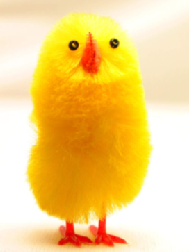
\includegraphics{chick}

\ifclasstoggle{timestamp}{with timestamp!}{}
%% Los cap'itulos inician con \chapter{T'itulo}, estos aparecen numerados y
%% se incluyen en el 'indice general.
%%
%% Recuerda que aqu'i ya puedes escribir acentos como: 'a, 'e, 'i, etc.
%% La letra n con tilde es: 'n.

\chapter{Introducci'on}\label{intro}
\providecommand\href[2]{#2}

Existen dos tipos de citas bibliograf'icas: usa \verb|\citep{..}| para
citas en \emph{par'entesis} y \verb|\citet{..}| para citas
en el \emph{texto}. Por ejemplo, estudios recientes han mostrado nuevos e
interesantes modelos que se pueden aplicar para reformular teor'ias
f'isicas~\citep{NewCam97}. Mientras que, el trabajo de \citet{Rofl06} fue
considerado muy divertido por una significativa fracci'on de la comunidad
de investigadores. Tambi'en es posible citar a varios trabajos en una sola
referencia \citep{Lamport86,Knuth84}.

Estos comandos para producir citas bibliograficas son provistos por
el paquete \textsf{natbib}. Para obtener m'as informaci'on, consulta la
documentaci'on de ese paquete~\citep{doc:natbib}. Por su parte, en
la documentaci\'on de \textsf{geometry} puedes encontrar detalles
adicionales sobre el sistema para ajustar los m'argenes del
documento~\citep{doc:geometry}. Lo que sigue
es un mont'on de texto sin sentido en lat'in que utilizaremos para llenar
algunas p'aginas.

\section{Random Latin Text}

Lorem ipsum dolor sit amet, consectetuer adipiscing elit. Integer arcu nisl,
consectetuer ut, vehicula nec, blandit id, nulla. Vestibulum in odio a odio
volutpat sollicitudin. Donec congue porta tellus. Ut quis est sed \href{http://www.example.com}{velit
blandit fringilla}. Nunc lobortis dui vitae sapien. In tincidunt magna eget
purus. Nam lorem quam, vehicula in, dictum et, congue eget, odio. Curabitur
gravida mi id dui. Aliquam erat volutpat. Fusce velit turpis, accumsan vel,
tincidunt at, aliquet at, sem. Cras viverra eros ac orci. Aenean vestibulum,
lorem sed luctus congue, arcu pede ultricies libero, at posuere felis nulla
et leo.

Fusce rhoncus lobortis orci. Quisque suscipit dolor. In tincidunt dictum
elit. Cras metus. Donec nibh mi, ornare a, ullamcorper in, gravida non,
augue. Aliquam erat volutpat. Aliquam commodo tellus sed dolor. Sed urna.
Phasellus blandit orci sit amet nulla. Fusce vel eros. Aenean ultrices
sodales mi. Aliquam erat volutpat. Fusce orci sem, sollicitudin convallis,
auctor a, sollicitudin vitae, dui. Sed massa. Duis luctus lectus ut lacus.

Morbi felis tellus, placerat quis, congue pretium, consectetuer at, tortor.
Nunc condimentum mattis urna. Donec dolor erat, fringilla ut, auctor ac,
vestibulum ut, velit. Aliquam convallis magna ac neque. Praesent varius
congue augue. Nulla adipiscing urna faucibus diam. Mauris porta sapien ut
justo. Donec suscipit tortor gravida ligula. Aliquam ac purus et massa
scelerisque vehicula. Maecenas a libero. Class aptent taciti sociosqu ad
litora torquent per conubia nostra, per inceptos himenaeos. Pellentesque
sit amet est eget metus tincidunt semper. Phasellus nec purus. Proin
venenatis lectus vel elit. Pellentesque augue quam, tincidunt sed, pretium
ut, feugiat id, odio. Aenean eu nibh et quam dignissim facilisis.

Suspendisse adipiscing. Maecenas tincidunt placerat justo. Ut mattis nunc ac
orci. Vestibulum quis velit sed massa vulputate posuere. Duis rhoncus lacus.
Quisque non lacus et nibh molestie tincidunt. Nulla tortor pede, auctor id,
eleifend sit amet, ultrices id, risus. Duis et lectus. Suspendisse interdum,
magna ut porta porta, quam tellus suscipit ligula, cursus consectetuer purus
erat et dolor. Phasellus venenatis, risus malesuada lacinia placerat, lectus
tellus lobortis ligula, eu porttitor tellus nibh eu enim. Morbi vel erat in
sem pharetra molestie. Duis tellus. In ipsum. Vivamus ac augue sed dui
hendrerit pulvinar. In dui erat, molestie ut, lacinia at, sagittis sed, nisi.
Maecenas libero. Nam volutpat dictum erat.

Fusce laoreet sapien ut lorem. Mauris sed leo a mi luctus sollicitudin.
Donec ornare nisi id dolor. Ut eros metus, tristique quis, ultrices ac,
accumsan cursus, est. Pellentesque mollis posuere sapien. Morbi nec augue.
Cum sociis natoque penatibus et magnis dis parturient montes, nascetur
ridiculus mus. Duis tristique, ipsum in tincidunt gravida, nunc nulla
vehicula felis, elementum eleifend nunc elit id magna. Cum sociis natoque
penatibus et magnis dis parturient montes, nascetur ridiculus mus. Curabitur
rhoncus dui ut sapien.

Sed orci. Nunc nisi lorem, convallis nec, porttitor at, porttitor et, erat.
Lorem ipsum dolor sit amet, consectetuer adipiscing elit. Donec luctus, velit
quis lacinia pulvinar, risus urna malesuada nisl, vel hendrerit erat enim ac
enim. Aliquam sapien dolor, fringilla quis, consequat auctor, sodales id,
est. In imperdiet est et dui. Cras libero lacus, feugiat a, auctor ut,
vulputate sollicitudin, orci. Ut tellus velit, rutrum tristique, eleifend sit
amet, auctor consectetuer, sapien. Fusce eget justo. Nam auctor lorem at
purus. Vestibulum ante ipsum primis in faucibus orci luctus et ultrices
posuere cubilia Curae; Pellentesque pretium enim sed tortor. Sed luctus velit
at ligula. Nunc id elit. Curabitur lacus. Mauris placerat nibh sit amet
turpis. Fusce varius, justo et ultrices dictum, urna risus rhoncus ipsum, sed
ultricies nunc arcu eu risus. Nam vitae purus.

Proin augue. Duis vehicula mauris sollicitudin sapien. Nam tristique lacus
nec nisl. Praesent quis enim. Vestibulum vel velit in purus luctus mattis.
Mauris ullamcorper tempor lorem. Quisque rutrum. Praesent enim nibh,
pellentesque non, lacinia accumsan, euismod a, lorem. Etiam fringilla
iaculis mauris. Aenean adipiscing purus in lacus. Maecenas quis nibh. Ut
non augue at mauris elementum luctus. Duis varius tincidunt mi. Aliquam
justo massa, auctor nec, malesuada interdum, mollis ac, mauris. Maecenas
ultricies gravida dui. Aliquam arcu elit, pretium eu, gravida ac, molestie
eu, enim. Etiam facilisis orci eget est. Integer eu orci non felis tincidunt
consectetuer. Sed imperdiet ultrices nibh.

%\include{capitulo1}
%\include{capitulo2}
%\include{capitulo3}
%\include{conclu}

\appendix
%% Cap'itulos incluidos despues del comando \appendix aparecen como ap'endices
%% de la tesis.
%\include{apendiceA}
%\include{apendiceB}
%\include{apendiceC}

%% Incluir la bibliograf'ia. Mirar el archivo "biblio.bib" para m'as detales
%% y un ejemplo.
\bibliography{biblio}

\end{document}
